
\section{Requirement Analysis}
\subsection{Functional Requirements}
\begin{table}[H]
\centering
\caption{Functional requirements}
\label{tab:fr}
\renewcommand{\arraystretch}{1.2}
\begin{tabular}{|c|p{11cm}|}
\hline
\textbf{ID} & \textbf{Description} \\
\hline
FR1 & Ingest PDF, image, and text study materials; chunk and index for student RAG. \\
\hline
FR2 & Answer student questions and summaries using retrieved public context only. \\
\hline
FR3 & Classify teacher-uploaded questions into six Bloom levels with confidence scores. \\
\hline
FR4 & Generate moderation text: reason and higher-level rewrite (GGUF). \\
\hline
FR5 & Block student queries/outputs that attempt to reconstruct protected exam content. \\
\hline
FR6 & Support federated training of privacy guard and teacher LoRA adapters. \\
\hline
\end{tabular}
\end{table}

\subsection{Non-Functional Requirements}
\begin{table}[H]
\centering
\caption{Non-functional requirements}
\label{tab:nfr}
\renewcommand{\arraystretch}{1.2}
\begin{tabular}{|c|p{11cm}|}
\hline
\textbf{ID} & \textbf{Description} \\
\hline
NFR1 & Offline operation; no mandatory cloud LLM API. \\
\hline
NFR2 & Peak model footprint under $\approx$1\,GB quantized weights (mmap). \\
\hline
NFR3 & CPU-only inference path for demo deployment. \\
\hline
NFR4 & Deterministic, auditable privacy decisions with logged risk scores. \\
\hline
NFR5 & Reproducible evaluation scripts writing JSON/CSV artifacts. \\
\hline
\end{tabular}
\end{table}

\section{System Overview / Architecture}
\subsection{High-Level Architecture}
Figure~\ref{fig:sysarch} shows the dual-role architecture: students use the RAG pipeline; teachers use Bloom moderation; both share a local Qwen backbone with role-specific adapters. A federated layer aggregates privacy-guard weights and teacher LoRA updates.

\begin{figure}[H]
    \centering
    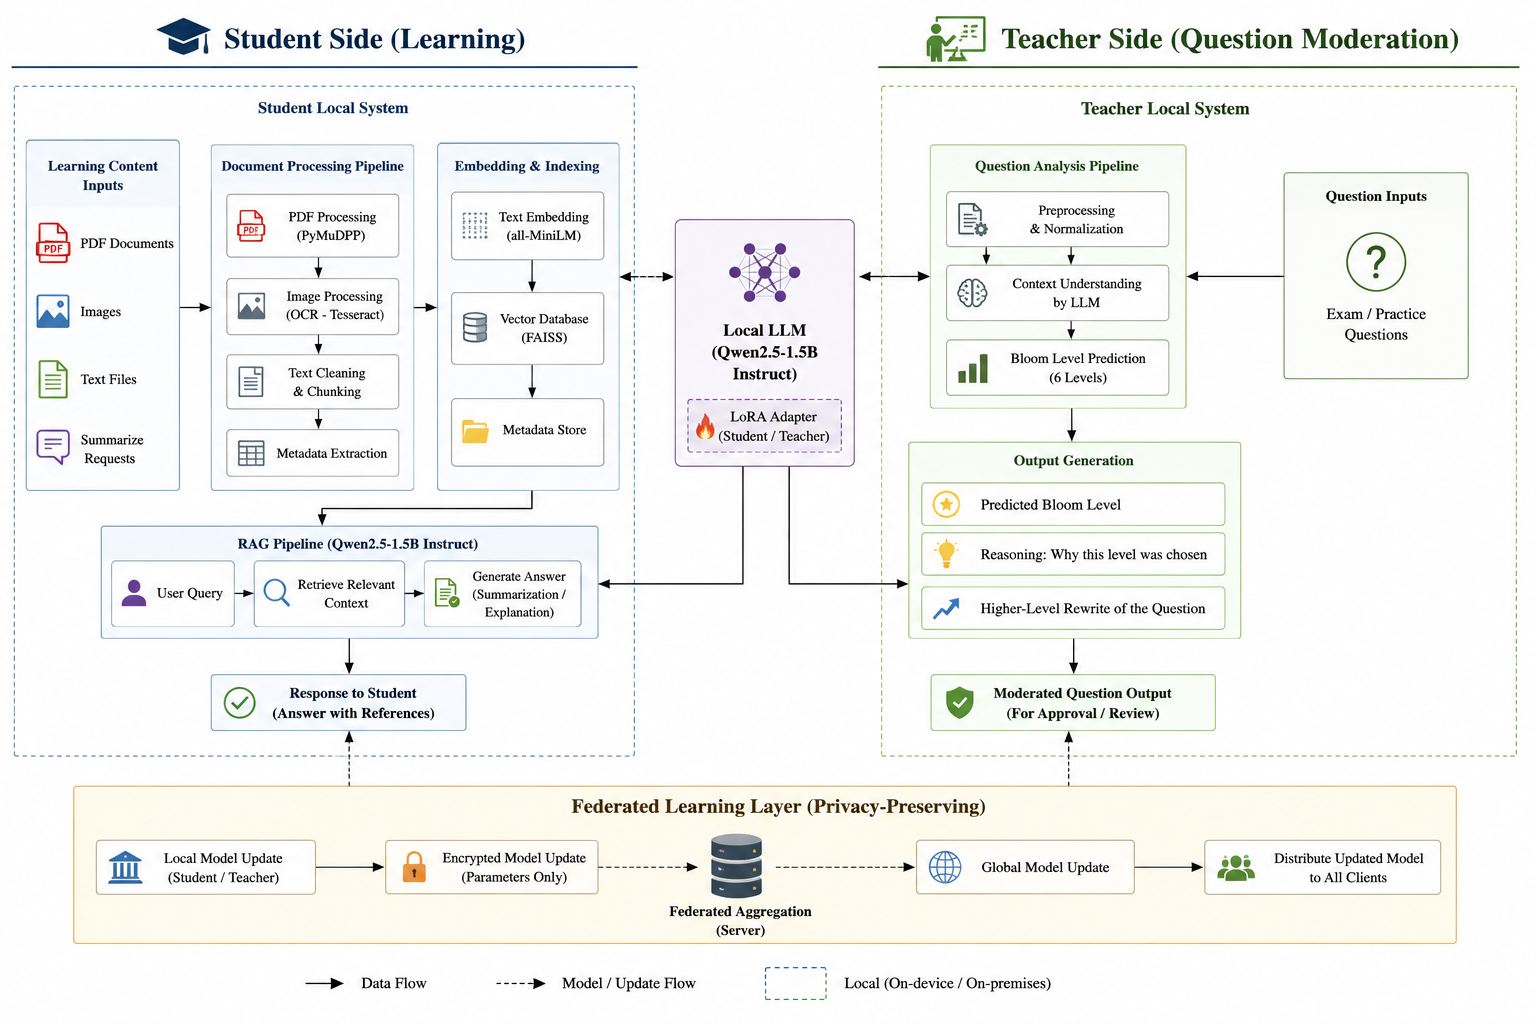
\includegraphics[width=0.95\linewidth]{images/system architecture (3).png}
    \caption{High-level system architecture (student RAG, teacher Bloom moderation, federated privacy layer)}
    \label{fig:sysarch}
\end{figure}

\subsection{Detailed Design Diagrams}
\begin{figure}[H]
    \centering
    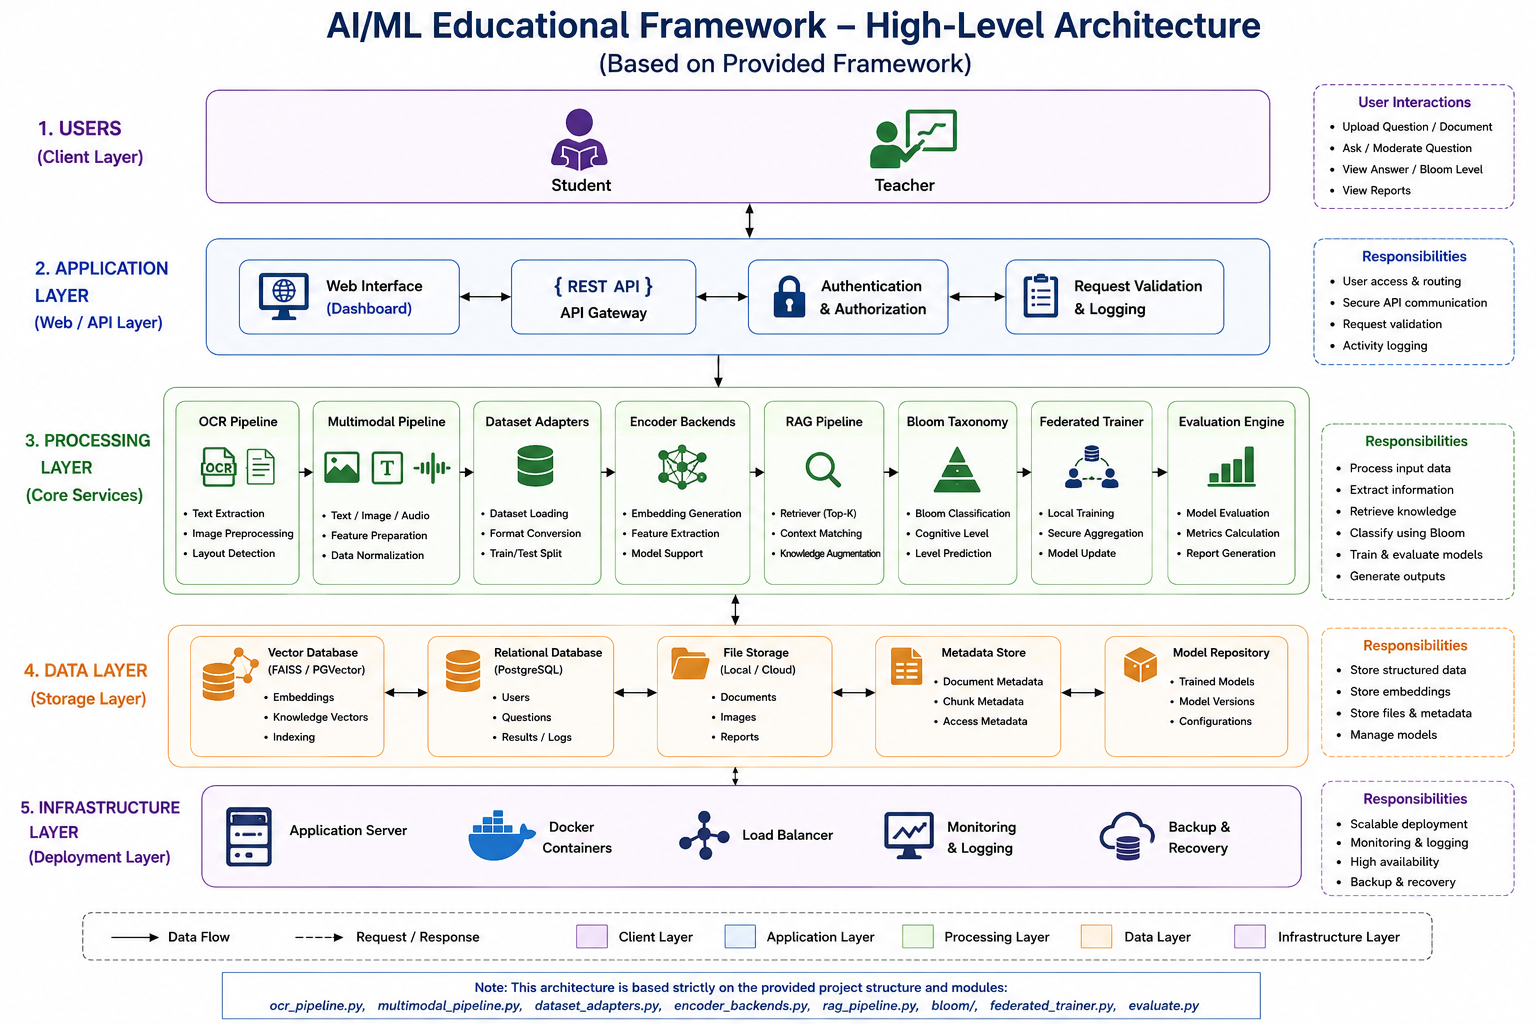
\includegraphics[width=0.85\linewidth]{images/high level architecture.png}
    \caption{High-level component view}
    \label{fig:highlevel}
\end{figure}

\begin{figure}[H]
    \centering
    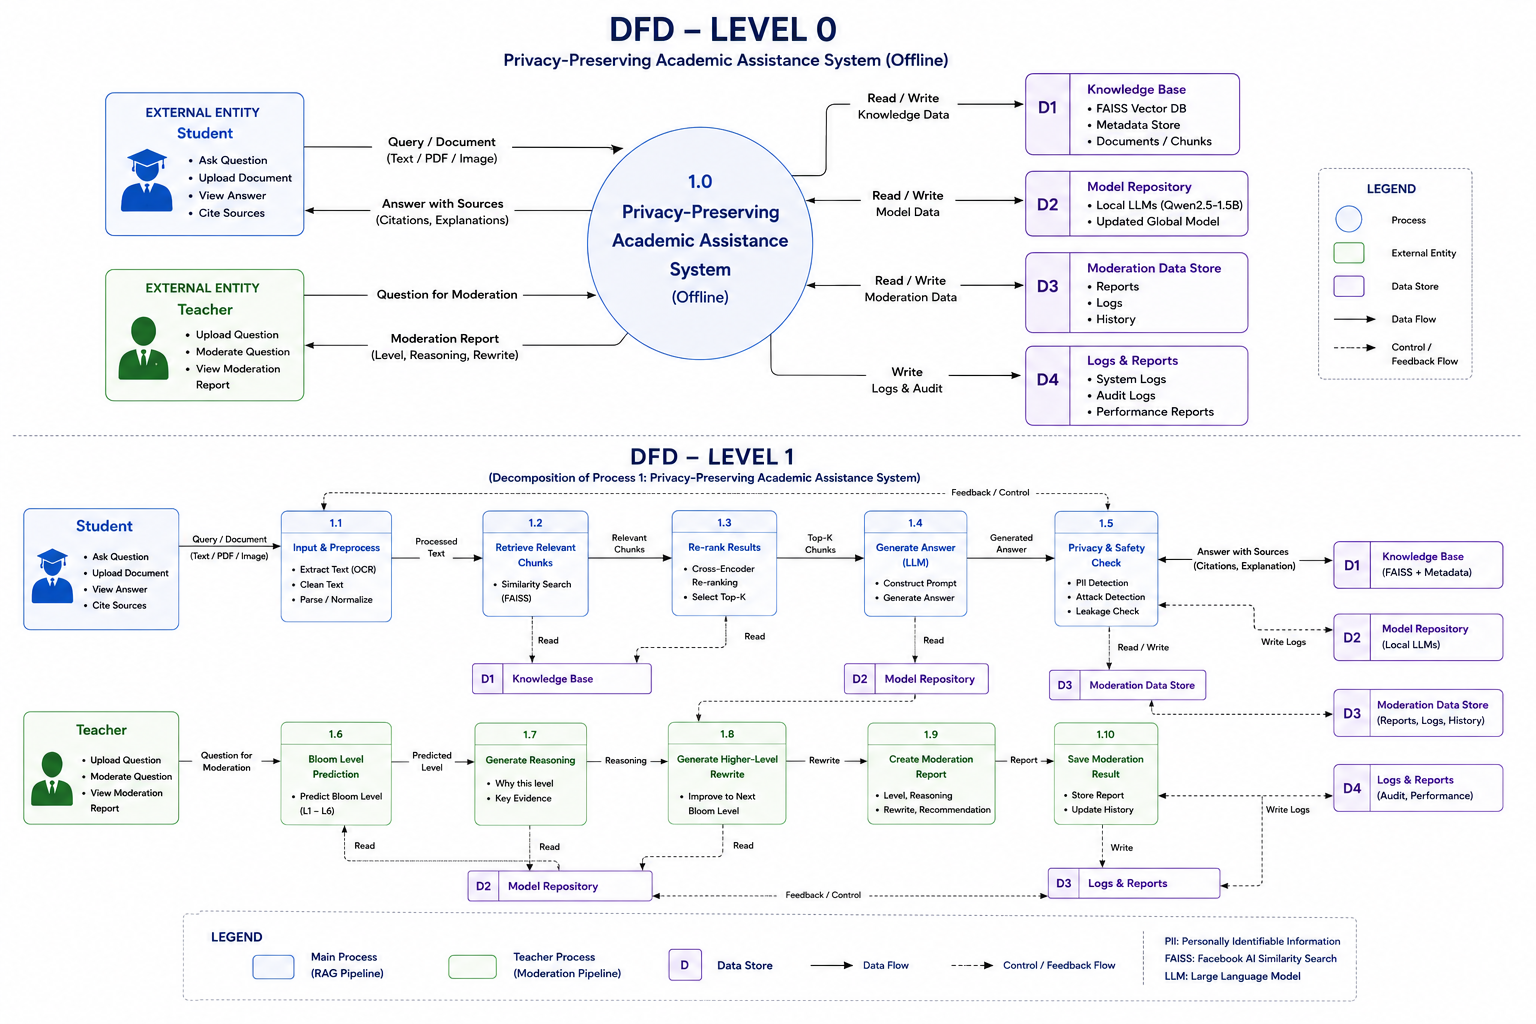
\includegraphics[width=0.9\linewidth]{images/DFD.png}
    \caption{Data flow among ingestion, retrieval, generation, and privacy modules}
    \label{fig:dfd}
\end{figure}

\begin{figure}[H]
    \centering
    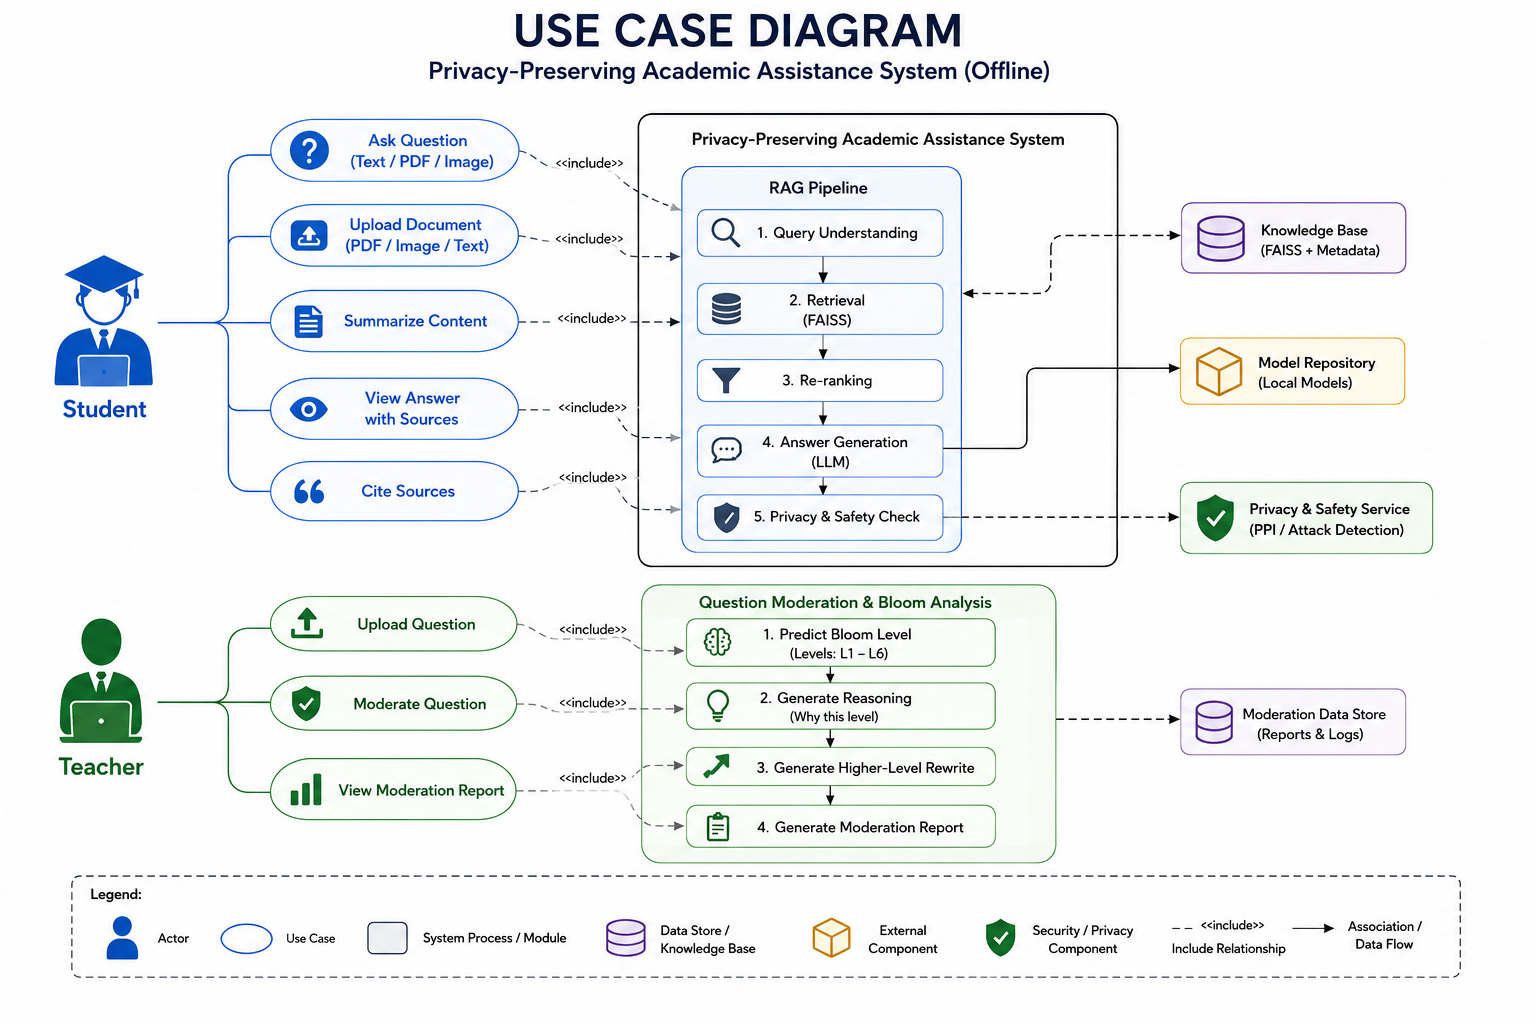
\includegraphics[width=0.9\linewidth]{images/use case diagram.png}
    \caption{Use cases for student and teacher roles}
    \label{fig:usecase}
\end{figure}

\subsection{Design Alternatives and Rationale}
A single cloud GPT endpoint was rejected due to privacy and cost. A monolithic shared index was rejected because it cannot isolate exam banks. The chosen design uses \textbf{separate public/protected stores}, \textbf{local GGUF inference}, and \textbf{layered privacy guard + federated risk model} for auditability.

\section{Algorithmic Flow / Pseudocode}
\begin{algorithm}[H]
\caption{Student RAG query (simplified)}
\begin{algorithmic}[1]
\State \textbf{Input:} query $q$, role $\leftarrow$ student
\State $C \leftarrow$ RetrievePublic($q$, FAISS, MiniLM)
\If{PrivacyGuard$(q, C, role)$ blocks}
   \State \Return refusal message
\EndIf
\State $b \leftarrow$ BloomLoRA$(q)$ \Comment{conditions generation style}
\State \Return QwenGGUF$(q, C, b)$
\end{algorithmic}
\end{algorithm}

\section{Summary}
Requirements, dual-corpus architecture, and role-separated flows provide the foundation for implementation in Chapter~\ref{cha:MethodologyAndImplementationU}.
